\section{Jonathan}
\subsection{Overview}
\begin{frame}{Jonathan: Overview}
\begin{itemize}
\item Collaborations
\item New Stuff
\end{itemize}
\end{frame}

\subsection{GUI Requirements Analysis}
\begin{frame}{GUI Requirements Analysis}
A collaboration between SW609, SW610 and SW612.\nl

A couple of the more noteworthy questions:
\begin{itemize}
\item How should switching from Guardian to Citizen and back happen?
\item Can there be multiple Guardians pr. Citizen?
\item Who are supposed to login?
\end{frame}

\begin{frame]{GUI Requirements Analysis}

Based on the userstories we were able to create the following requirements for the Launcher:



\end{frame}

\subsection{REST Collaboration}
\begin{frame}{REST Collaboration}
A Collaboration between SW609, SW610, SW613 and SW614.\nl


\begin{itemize}
\item 


\end{itemize}
\end{frame}



% \subsection{Network Structure}
% \begin{frame}{Network Structure}
% \begin{itemize}
% \item What does the network look like?
% \item Which features are used and how are their domains defined?
% \end{itemize}
% \begin{figure}
%   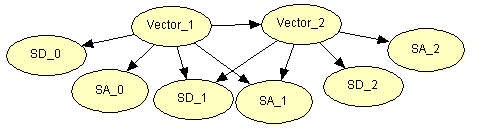
\includegraphics[scale=0.8]{figures/BNDone.PNG}
% \end{figure}
% \end{frame}
